%\documentclass[border=2pt]{standalone}
\documentclass{article}

\usepackage{tikz}
\usetikzlibrary{matrix,positioning,arrows.meta,arrows}

\tikzset{
mymat/.style={
  matrix of math nodes,
  text height=2.5ex,
  text depth=0.75ex,
  text width=3.25ex,
  align=center,
  column sep=-\pgflinewidth
  },
mymats/.style={
  mymat,
  nodes={draw,fill=#1}
  }  
}

\begin{document}


Komplex:




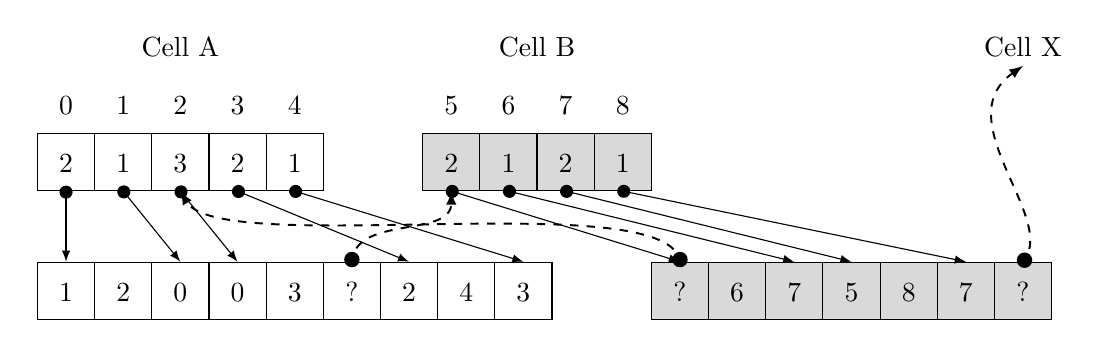
\begin{tikzpicture}[>=latex]
\matrix[mymat,anchor=west,row 2/.style={nodes=draw}]
at (0,0) 
(mat1)
{
0 & 1 & 2 & 3 & 4 \\
2 & 1 & 3 & 2 & 1 \\
};
\matrix[mymat,right=of mat1,row 2/.style={nodes={draw,fill=gray!30}}]
(mat2)
{
5 & 6 & 7 & 8 \\
2 & 1 & 2 & 1 \\
};
\matrix[mymats=white,anchor=west]
at (0,-2) 
(mat3)
{
1 & 2 & 0 & 0 & 3 & ? & 2 & 4 & 3 \\
};
\matrix[mymats=gray!30,right=of mat3]
(mat4)
{
? & 6 & 7 & 5 & 8 & 7 & ? \\
};

\node[above=0pt of mat1]
  (cella) {Cell A};
\node[above=0pt of mat2]
  (cellb) {Cell B};
\node at (mat4-1-7.north|-cellb)
  (cellx) {Cell X};

\begin{scope}[shorten <= -2pt]
\draw[*->]
  (mat1-2-1.south) -- (mat3-1-1.north);
\draw[*->]
  (mat1-2-2.south) -- (mat3-1-3.north);
\draw[*->]
  (mat1-2-3.south) -- (mat3-1-4.north);
\draw[*->]
  (mat1-2-4.south) -- (mat3-1-7.north);
\draw[*->]
  (mat1-2-5.south) -- (mat3-1-9.north);

\draw[*->]
  (mat2-2-1.south) -- (mat4-1-1.north);
\draw[*->]
  (mat2-2-2.south) -- (mat4-1-3.north);
\draw[*->]
  (mat2-2-3.south) -- (mat4-1-4.north);
\draw[*->]
  (mat2-2-4.south) -- (mat4-1-6.north);

\draw[*->,dashed,line width=0.7pt]
  (mat4-1-1.north) to[out=90,in=-60,looseness=0.4] (mat1-2-3.south);
\draw[*->,dashed,line width=0.7pt]
  (mat3-1-6.north) to[out=90,in=-90] (mat2-2-1.south);
\draw[*->,dashed,line width=0.7pt]
  (mat4-1-7.north) ..
    controls ++ (0.5,0.5) and ++(-1,-0.7) ..  
  (cellx.south);
\end{scope}
\end{tikzpicture}

\bigskip

Etwas einfacher: \\


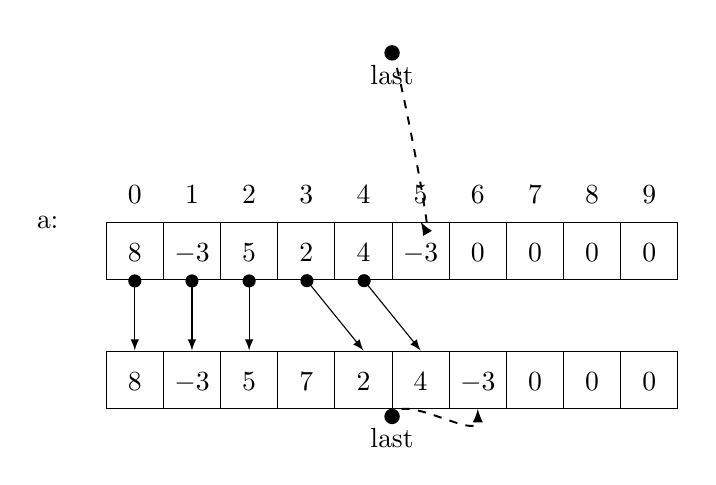
\begin{tikzpicture}[>=latex]
\matrix[mymat,anchor=west,row 2/.style={nodes=draw}]
at (0,0) 
(mat1)
{
0 & 1 & 2 & 3 & 4 & 5 & 6 & 7 & 8 & 9  \\
8 & -3 & 5 & 2 & 4 & -3 & 0 & 0 & 0 & 0 \\
};

\matrix[mymats=white,anchor=west]
at (0,-2) 
(mat3)
{
8 & -3 & 5 & 7 & 2 & 4 & -3 & 0 & 0 & 0    \\
};


\node[above=22pt of mat1] (last1) {last};

\node[below=0pt of mat3] (last3) {last};

\node[left=10pt of mat1] (a1) {a:};

\begin{scope}[shorten <= -2pt]
\draw[*->]
  (mat1-2-1.south) -- (mat3-1-1.north);
\draw[*->]
  (mat1-2-2.south) -- (mat3-1-2.north);
\draw[*->]
  (mat1-2-3.south) -- (mat3-1-3.north);
\draw[*->]
  (mat1-2-4.south) -- (mat3-1-5.north);
\draw[*->]
  (mat1-2-5.south) -- (mat3-1-6.north);


\draw[*->,dashed,line width=0.7pt] (last1) to[out=90,in=-60,looseness=0.4] (mat1-2-6.north);
\draw[*->,dashed,line width=0.7pt] (last3) to[out=90,in=-90] (mat3-1-7.south);

\end{scope}
\end{tikzpicture}


Arrays 0: \\ \bigskip

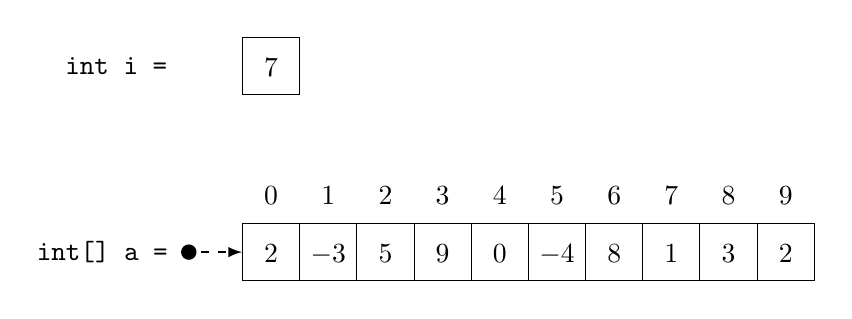
\begin{tikzpicture}[>=latex]

\matrix[mymats=white,anchor=west,row 2/.style={nodes=draw}]
at (0,0) 
(mat0)
{
7 \\
};


\matrix[mymat,anchor=west,row 2/.style={nodes=draw}]
at (0,-2) 
(mat1)
{
0 & 1 & 2 & 3 & 4 & 5 & 6 & 7 & 8 & 9  \\
2 & -3 & 5 & 9 & 0 & -4 & 8 & 1 & 3 & 2 \\
};




\node[left=20pt of mat0] (a0) {\texttt{int i = }};
\node[left=20pt of mat1-2-1] (a1) {\texttt{int[] a =}~~};

\begin{scope}[shorten <= -2pt]


\draw[*->,dashed,line width=0.7pt] (a1.east) to (mat1-2-1.west);


\end{scope}
\end{tikzpicture}


\bigskip
Bsp1: \\ \bigskip


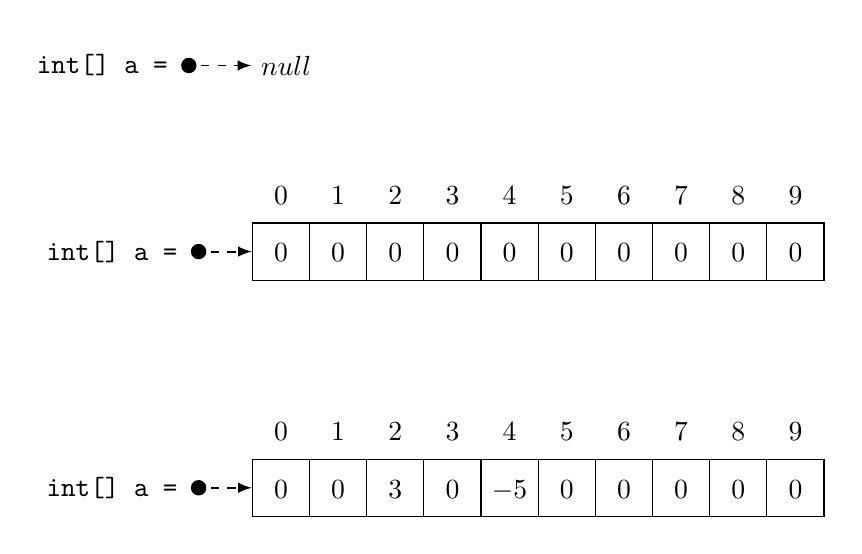
\begin{tikzpicture}[>=latex]

\matrix[mymat,anchor=west,row 2/.style={nodes=draw}]
at (0,0) 
(mat0)
{
null \\
};


\matrix[mymat,anchor=west,row 2/.style={nodes=draw}]
at (0,-2) 
(mat1)
{
0 & 1 & 2 & 3 & 4 & 5 & 6 & 7 & 8 & 9  \\
0 & 0 & 0 & 0 & 0 & 0 & 0 & 0 & 0 & 0 \\
};
 
\matrix[mymat,anchor=west,row 2/.style={nodes=draw}]
at (0,-5) 
(mat3)
{
0 & 1 & 2 & 3 & 4 & 5 & 6 & 7 & 8 & 9  \\
0 & 0 & 3 & 0 & -5 & 0 & 0 & 0 & 0 & 0 \\
};



\node[left=20pt of mat0] (a0) {\texttt{int[] a =}~~};
\node[left=20pt of mat1-2-1] (a1) {\texttt{int[] a =}~~};
\node[left=20pt of mat3-2-1] (a3) {\texttt{int[] a =}~~};

\begin{scope}[shorten <= -2pt]


\draw[*->,dashed,line width=0.7pt] (a0.east) to (mat0-1-1.west);
\draw[*->,dashed,line width=0.7pt] (a1.east) to (mat1-2-1.west);
\draw[*->,dashed,line width=0.7pt] (a3.east) to (mat3-2-1.west);


\end{scope}
\end{tikzpicture}


Bsp2: \\


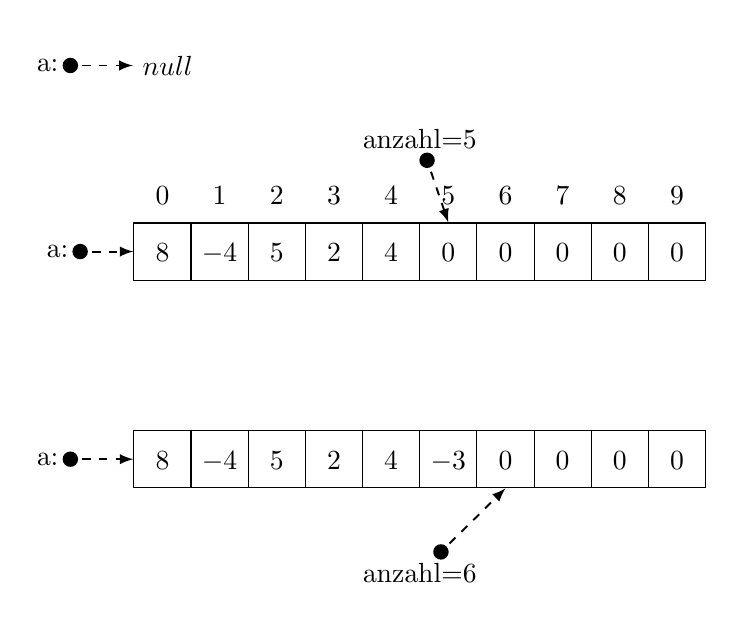
\begin{tikzpicture}[>=latex]

\matrix[mymat,anchor=west,row 2/.style={nodes=draw}]
at (0,0) 
(mat0)
{
null \\
};


\matrix[mymat,anchor=west,row 2/.style={nodes=draw}]
at (0,-2) 
(mat1)
{
0 & 1 & 2 & 3 & 4 & 5 & 6 & 7 & 8 & 9  \\
8 & -4 & 5 & 2 & 4 & 0 & 0 & 0 & 0 & 0 \\
};

\matrix[mymats=white,anchor=west]
at (0,-5) 
(mat3)
{
8 & -4 & 5 &  2 & 4 & -3 & 0 & 0 & 0 & 0    \\
};


\node[above=-1pt of mat1] (last1) {anzahl=5};

\node[below=20pt of mat3] (last3) {anzahl=6};

\node[left=20pt of mat0] (a0) {a:};
\node[left=20pt of mat1-2-1] (a1) {a:};
\node[left=20pt of mat3] (a3) {a:};

\begin{scope}[shorten <= -2pt]


\draw[*->,dashed,line width=0.7pt] (a0.east) to (mat0-1-1.west);
\draw[*->,dashed,line width=0.7pt] (a1.east) to (mat1-2-1.west);
\draw[*->,dashed,line width=0.7pt] (a3.east) to (mat3-1-1.west);

\draw[*->,dashed,line width=0.7pt] (last1) to (mat1-2-6.north);
\draw[*->,dashed,line width=0.7pt] (last3) to (mat3-1-7.south);

\end{scope}
\end{tikzpicture}

Bsp3: \\


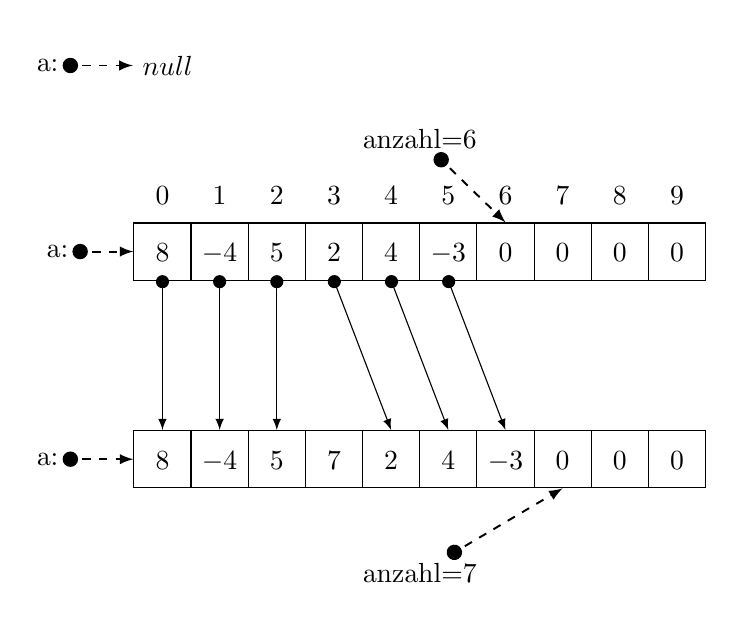
\begin{tikzpicture}[>=latex]

\matrix[mymat,anchor=west,row 2/.style={nodes=draw}]
at (0,0) 
(mat0)
{
null \\
};


\matrix[mymat,anchor=west,row 2/.style={nodes=draw}]
at (0,-2) 
(mat1)
{
0 & 1 & 2 & 3 & 4 & 5 & 6 & 7 & 8 & 9  \\
8 & -4 & 5 & 2 & 4 & -3 & 0 & 0 & 0 & 0 \\
};

\matrix[mymats=white,anchor=west]
at (0,-5) 
(mat3)
{
8 & -4 & 5 & 7 & 2 & 4 & -3 & 0 & 0 & 0    \\
};


\node[above=-1pt of mat1] (last1) {anzahl=6};

\node[below=20pt of mat3] (last3) {anzahl=7};

\node[left=20pt of mat0] (a0) {a:};
\node[left=20pt of mat1-2-1] (a1) {a:};
\node[left=20pt of mat3] (a3) {a:};

\begin{scope}[shorten <= -2pt]
\draw[*->] (mat1-2-1.south) -- (mat3-1-1.north);
\draw[*->] (mat1-2-2.south) -- (mat3-1-2.north);
\draw[*->] (mat1-2-3.south) -- (mat3-1-3.north);
\draw[*->] (mat1-2-4.south) -- (mat3-1-5.north);
\draw[*->] (mat1-2-5.south) -- (mat3-1-6.north);
\draw[*->] (mat1-2-6.south) -- (mat3-1-7.north);

\draw[*->,dashed,line width=0.7pt] (a0.east) to (mat0-1-1.west);
\draw[*->,dashed,line width=0.7pt] (a1.east) to (mat1-2-1.west);
\draw[*->,dashed,line width=0.7pt] (a3.east) to (mat3-1-1.west);

\draw[*->,dashed,line width=0.7pt] (last1) to (mat1-2-7.north);
\draw[*->,dashed,line width=0.7pt] (last3) to (mat3-1-8.south);

\end{scope}
\end{tikzpicture}



\end{document}
